\documentclass[../main.tex]{subfiles}
\begin{document}

%\begin{figure}[H]
%    \centering
%    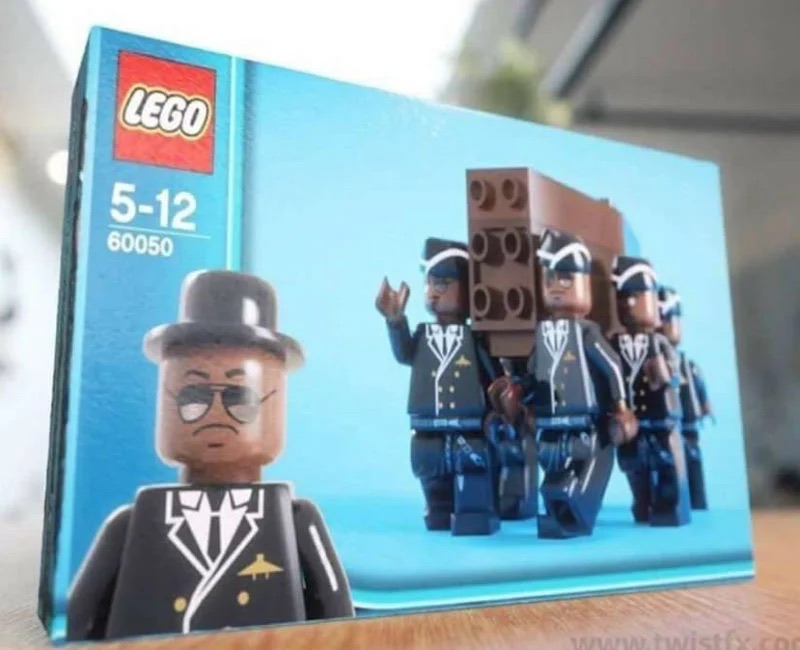
\includegraphics[width=10cm]{Bilddateien/CoffinDance.jpg}
%    \label{fig:myfreshbild}
%\end{figure}

In this experiment, the nuclear magnetic resonance (NMR) is studied in a simple water probe. Firstly, parameters for a clear resonance signal are investigated (excitation signal freqency, length etc.). Using this signal, the relaxation times for spin-lattice- and spin-spin-relaxtion are measured. In the process of this, typical NMR-pulse sequences are familiarized: namley, the spin-echo and Carr-Purcell-Meiboom-Gill (CPMG) sequence. Furthermore, the effects of different ion-solutions on the spatial contrast of relaxation times are studied. Lastly, one- and twodimensional images displaying the distribution of nuclear spins are recored.

\end{document}